% Implementation flow on the Gazebo X3 (gazebo.py v2 / x3_sim), blocks 7-10.
% Build:  pdflatex flow_x3.tex
\documentclass[border=10pt]{standalone}
\usepackage{tikz}
% Shared preamble of the two flow diagrams (flow_paper.tex, flow_x3.tex)
\usepackage{amsmath,amssymb,bm}
\usepackage[most]{tcolorbox}
\usetikzlibrary{positioning,arrows.meta,calc,fit,backgrounds}
\definecolor{cPlant}{HTML}{37474F}
\definecolor{cEnv}{HTML}{A0620F}
\definecolor{cCtrl}{HTML}{AD1457}
\definecolor{cAdapt}{HTML}{4527A0}
\definecolor{cX3}{HTML}{1565C0}
\definecolor{cOk}{HTML}{2E7D32}
\definecolor{cText}{HTML}{263238}
\definecolor{cRef}{HTML}{546E7A}
\newcommand{\vq}{\bm{q}}  \newcommand{\qv}{\bm{q}_v} \newcommand{\vw}{\bm{\omega}}
\newcommand{\vu}{\bm{u}}  \newcommand{\vd}{\bm{d}}   \newcommand{\vs}{\bm{s}}
\newcommand{\vtau}{\bm{\tau}} \newcommand{\veps}{\bm{\varepsilon}} \newcommand{\vF}{\bm{F}}
\newcommand{\vp}{\bm{p}}  \newcommand{\vv}{\bm{v}}
\newcommand{\that}{\hat{\theta}}
\newcommand{\sat}{\operatorname{sat}}
\newcommand{\R}{\mathbb{R}}
% \fblock{name}{position}{colour}{number}{title}{equations}{IN}{OUT}
\newcommand{\fblock}[8]{%
  \node[inner sep=0pt, outer sep=0pt] (#1) at #2 {%
  \begin{tcolorbox}[enhanced, width=8.4cm, colback=white, colframe=#3, colbacktitle=#3, coltitle=white,
     title={\sffamily\bfseries\small\tcbox[on line, colback=white, colframe=white, colupper=#3, arc=5pt,
     boxsep=0pt, left=2.5pt, right=2.5pt, top=0.5pt, bottom=0.5pt]{#4}\ #5}, boxrule=0.8pt, arc=3pt,
     left=5pt, right=5pt, top=4pt, bottom=4pt, colbacklower=#3!7, segmentation style={draw=#3!45},
     fontupper=\small, fontlower=\scriptsize\sffamily\color{cText}]
  \centering #6
  \tcblower\raggedright\textbf{IN}\enspace #7\par\smallskip\textbf{OUT}\enspace #8
  \end{tcolorbox}};}
\tikzset{
  sig/.style={-{Stealth[length=2.6mm]}, line width=0.9pt, color=cText},
  lbl/.style={font=\scriptsize\sffamily, text=cText, fill=white, inner sep=1.6pt, align=center},
  aux/.style={draw=cRef, fill=cRef!6, rounded corners=3pt, line width=0.7pt,
              font=\scriptsize\sffamily, text=cText, align=center, inner sep=5pt},
}

\begin{document}
\sffamily
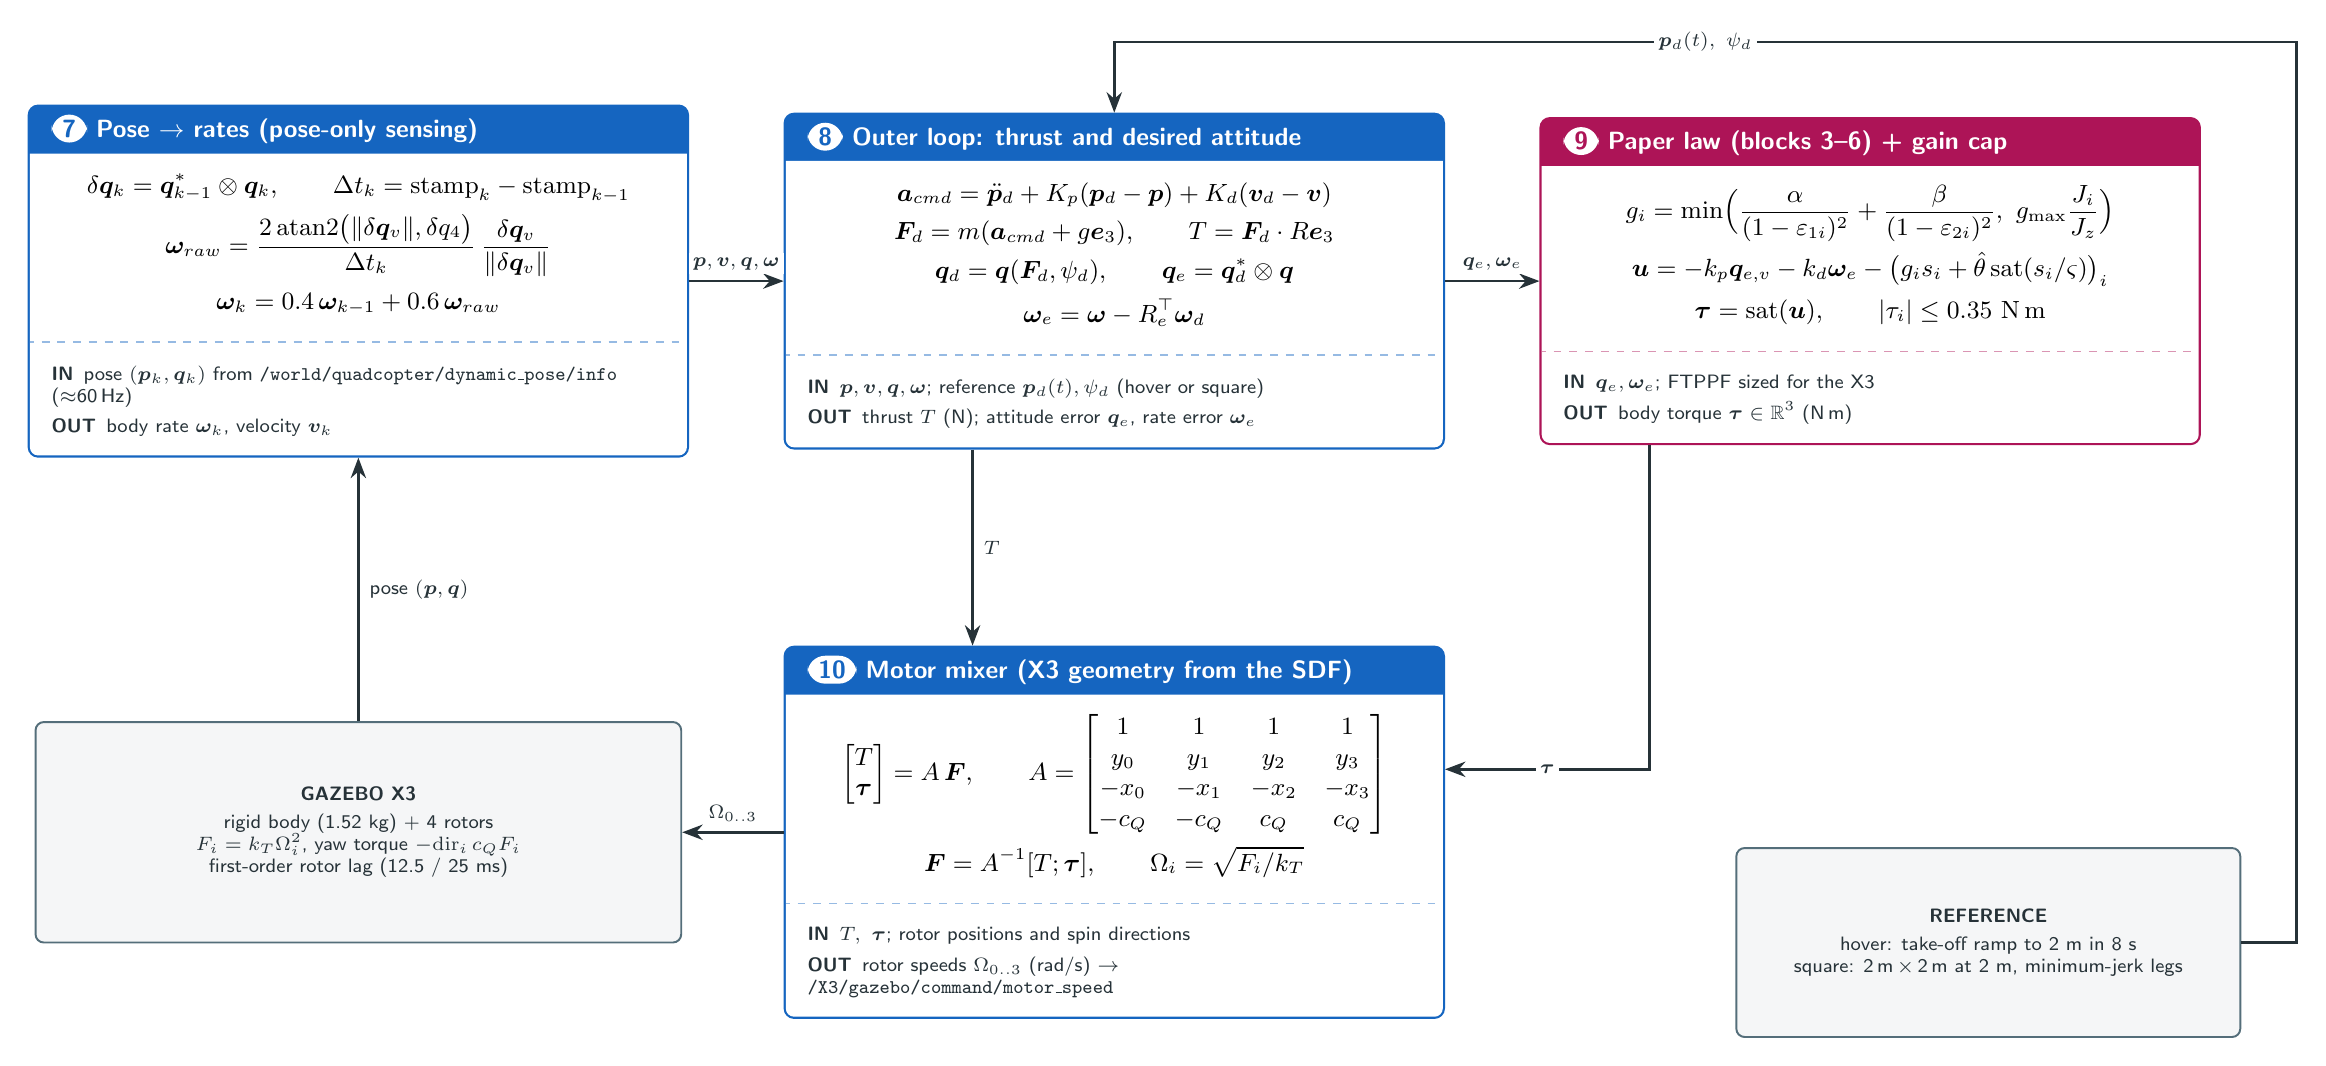
\begin{tikzpicture}
\fblock{b7}{(0,0)}{cX3}{7}{Pose $\rightarrow$ rates (pose-only sensing)}{%
  $\begin{gathered}\delta\vq_k=\vq_{k-1}^{*}\otimes\vq_k,\qquad \Delta t_k=\text{stamp}_k-\text{stamp}_{k-1}\\
   \vw_{raw}=\dfrac{2\,\mathrm{atan2}\big(\|\delta\vq_v\|,\delta q_4\big)}{\Delta t_k}\,\dfrac{\delta\vq_v}{\|\delta\vq_v\|}\\
   \vw_k=0.4\,\vw_{k-1}+0.6\,\vw_{raw}\end{gathered}$}
  {pose $(\vp_k,\vq_k)$ from \texttt{/world/quadcopter/dynamic\_pose/info} ($\approx$60\,Hz)}
  {body rate $\vw_k$, velocity $\vv_k$}
\fblock{b8}{(9.6,0)}{cX3}{8}{Outer loop: thrust and desired attitude}{%
  $\begin{gathered}\bm a_{cmd}=\ddot{\vp}_d+K_p(\vp_d-\vp)+K_d(\vv_d-\vv)\\
   \vF_d=m(\bm a_{cmd}+g\bm e_3),\qquad T=\vF_d\cdot R\bm e_3\\
   \vq_d=\vq(\vF_d,\psi_d),\qquad \vq_e=\vq_d^{*}\otimes\vq\\
   \vw_e=\vw-R_e^{\top}\vw_d\end{gathered}$}
  {$\vp,\vv,\vq,\vw$; reference $\vp_d(t),\psi_d$ (hover or square)}
  {thrust $T$ (N); attitude error $\vq_{e}$, rate error $\vw_e$}
\fblock{b9}{(19.2,0)}{cCtrl}{9}{Paper law (blocks 3--6) + gain cap}{%
  $\begin{gathered}g_i=\min\!\Big(\dfrac{\alpha}{(1-\varepsilon_{1i})^2}+\dfrac{\beta}{(1-\varepsilon_{2i})^2},\ g_{\max}\dfrac{J_i}{J_z}\Big)\\
   \vu=-k_p\vq_{e,v}-k_d\vw_e-\big(g_i s_i+\that\sat(s_i/\varsigma)\big)_i\\
   \vtau=\sat(\vu),\qquad |\tau_i|\le 0.35\ \text{N\,m}\end{gathered}$}
  {$\vq_{e},\vw_e$; FTPPF sized for the X3}
  {body torque $\vtau\in\R^3$ (N\,m)}
\fblock{b10}{(9.6,-7.0)}{cX3}{10}{Motor mixer (X3 geometry from the SDF)}{%
  $\begin{gathered}\begin{bmatrix}T\\ \vtau\end{bmatrix}=A\,\vF,\qquad
   A=\begin{bmatrix}1&1&1&1\\ y_0&y_1&y_2&y_3\\ -x_0&-x_1&-x_2&-x_3\\ -c_Q&-c_Q&c_Q&c_Q\end{bmatrix}\\
   \vF=A^{-1}[T;\vtau],\qquad \Omega_i=\sqrt{F_i/k_T}\end{gathered}$}
  {$T,\ \vtau$; rotor positions and spin directions}
  {rotor speeds $\Omega_{0..3}$ (rad/s) $\rightarrow$ \texttt{/X3/gazebo/command/motor\_speed}}
\node[aux, minimum width=8.2cm, minimum height=2.8cm] (gz) at (0,-7.0)
  {\textbf{GAZEBO X3}\\[2pt] rigid body (1.52 kg) + 4 rotors\\ $F_i=k_T\Omega_i^2$, yaw torque $-\mathrm{dir}_i\,c_Q F_i$\\ first-order rotor lag (12.5 / 25 ms)};
\node[aux, minimum width=6.4cm, minimum height=2.4cm] (ref) at (20.7,-8.4)
  {\textbf{REFERENCE}\\[2pt] hover: take-off ramp to 2 m in 8 s\\ square: 2\,m\,$\times$\,2\,m at 2 m, minimum-jerk legs};
\draw[sig] (gz.north) -- node[lbl, right=2pt]{pose $(\vp,\vq)$} (b7.south);
\draw[sig] (b7.east) -- node[lbl, above=2pt]{$\vp,\vv,\vq,\vw$} (b8.west);
\draw[sig] (b8.east) -- node[lbl, above=2pt]{$\vq_e,\vw_e$} (b9.west);
\draw[sig] (ref.east) -- ++(0.7,0) |- node[lbl, pos=0.75]{$\vp_d(t),\ \psi_d$} ($(b8.north)+(0,0.9)$) -- (b8.north);
\draw[sig] ($(b9.south)+(-2.8,0)$) |- node[lbl, pos=0.75]{$\vtau$} ($(b10.east)+(0,0.8)$);
\draw[sig] ($(b8.south)+(-1.8,0)$) -- node[lbl, right=2pt]{$T$} ($(b10.north)+(-1.8,0)$);
\draw[sig] (b10.west) -- node[lbl, above=2pt]{$\Omega_{0..3}$} (gz.east);
\end{tikzpicture}
\end{document}
